% =====================================================================
% Predicción de la duración de desvíos de ruta · Lab. de IA · TP1 · Grupo 5
% Presentación formal (Beamer, 16:9).
%
% Overleaf: subir la carpeta completa (main.tex, tema-formal.sty, img/ y
% figuras/) y compilar con pdfLaTeX (Menú > Compiler > pdfLaTeX).
%
% Los gráficos de figuras/*.pdf salen de los datos de Tecfield con
% figuras/generar_figuras.py (corre el notebook del proyecto); los diagramas
% están dibujados con TikZ en este archivo.
% =====================================================================
\documentclass[aspectratio=169,10pt]{beamer}
\usepackage{tema-formal}

\title[Predicción de la duración de desvíos de ruta]{Predicción de la duración de desvíos de ruta\\en flotas de transporte de personal}
\subtitle{Trabajo Práctico Obligatorio N.\textsuperscript{o}~1 · Proyecto con Tecfield}
\author[Grupo 5 · Reibold, Fernandez Gramajo, Kissner]{Sebastián Reibold \and Bautista Fernandez Gramajo \and Davor Kissner}
\institute{Laboratorio de Inteligencia Artificial · Facultad de Informática · Universidad Nacional del Comahue}
\date{26 de noviembre de 2026}

\begin{document}

% =====================================================================
% PORTADA
% =====================================================================
{\setbeamertemplate{footline}{}
\begin{frame}[plain,noframenumbering]
\begin{tikzpicture}[remember picture,overlay,shift={(current page.north west)},y=-1cm]
  \fill[azul] (0,0) rectangle (16,0.3);
  \fill[celeste] (0,0.3) rectangle (16,0.35);
  \node[anchor=west] at (0.8,1.25) {
\includegraphics[height=1.15cm]{img/logo-fai.png}};
  \node[anchor=east] at (15.2,1.25) {
\includegraphics[height=1.15cm]{img/logo-uncoma.png}};
  \node[align=center,text=gris,font=\small] at (8,1.25) {Universidad Nacional del Comahue\\Facultad de Informática\\Laboratorio de Inteligencia Artificial};
  \node[align=center,text=azul,font=\LARGE\bfseries] at (8,2.95) {Predicción de la duración de desvíos de ruta};
  \node[align=center,text=azul,font=\Large] at (8,3.65) {en flotas de transporte de personal};
  \fill[celeste] (5.5,4.15) rectangle (10.5,4.18);
  \node[align=center,font=\normalsize] at (8,4.6) {Trabajo Práctico Obligatorio N.\textsuperscript{o}~1 · Proyecto con Tecfield};
  \node[anchor=north,font=\small] at (8,5.2) {%
    \begin{tabular}{@{}ll@{}}
      \toprule
      \textbf{Integrante} & \textbf{Legajo} \\
      \midrule
      Reibold, Sebastián Alejandro & FAI-3854 \\
      Fernandez Gramajo, Bautista & FAI-3874 \\
      Kissner, Davor & FAI-3185 \\
      \bottomrule
    \end{tabular}};
  \node[text=gris,font=\small] at (8,8.0) {Grupo 5 · Cursado 2026 · 26 de noviembre de 2026};
  \fill[azul] (0,8.75) rectangle (16,9);
\end{tikzpicture}
\end{frame}}

% =====================================================================
\begin{frame}{Contenido}
  \tableofcontents[hideallsubsections]
\end{frame}

% =====================================================================
\section{Problema y objetivo}
% =====================================================================
\begin{frame}{Contexto: desvíos de ruta en Tecfield}
\begin{columns}[T,onlytextwidth]
\begin{column}{0.47\textwidth}
  \begin{itemize}\setlength{\itemsep}{5pt}
    \item Tecfield traslada personal a obras y yacimientos.
    \item Cada viaje tiene una \textbf{hoja de ruta} con el recorrido planificado.
    \item Si el vehículo se aleja más de \textbf{500\,m} de ese recorrido, un detector registra un \textbf{desvío}.
    \item \textbf{\T} es el primer punto fuera de ruta: el momento en que salta la alerta. Ahí nadie sabe si el vehículo vuelve en un minuto o en una hora.
    \item Hoy todas las alertas se atienden con la misma prioridad.
  \end{itemize}
\end{column}
\begin{column}{0.5\textwidth}
  \centering
  \begin{tikzpicture}[x=0.78cm,y=0.78cm,font=\scriptsize]
    \def\ruta{(0,3.2) .. controls (1.4,3.3) and (2.2,2.1) .. (3.9,2.0) .. controls (5.6,1.9) and (6.4,0.9) .. (8.2,0.7)}
    \draw[line width=16pt,celeste!35] \ruta;
    \draw[line width=1.8pt,azul] \ruta;
    \draw[rojo,line width=1.3pt] plot[smooth] coordinates {(4.3,1.98) (4.7,2.7) (5.3,3.2) (6.0,3.25) (6.6,2.6) (6.9,1.6) (7.05,0.9)};
    \foreach \p in {(4.7,2.7),(5.3,3.2),(6.0,3.25),(6.6,2.6),(6.9,1.6)}{\fill[rojo] \p circle (0.07);}
    \draw[rojo,line width=0.8pt] (4.7,2.7) circle (0.18);
    \draw[azul,fill=white,line width=1pt] (0,3.2) circle (0.13);
    \fill[azul] (8.05,0.55) rectangle (8.35,0.85);
    \node[anchor=south west,gris] at (-0.2,3.35) {Base};
    \node[anchor=north,azul] at (8.2,0.5) {Obra};
    \node[anchor=north,azul] at (2.2,1.95) {Hoja de ruta};
    \node[gris,anchor=north] at (4.6,1.45) {banda de 500\,m};
    \node[anchor=east,rojo,font=\scriptsize\bfseries] at (4.5,3.25) {\T: primer ping};
    \draw[rojo,line width=0.5pt] (4.5,3.15) -- (4.62,2.85);
    \node[anchor=west,rojo] at (7.15,2.4) {desvío};
  \end{tikzpicture}
  \fuente{Esquema ilustrativo: la línea azul es el recorrido planificado y los puntos rojos, las lecturas de desvío.}
\end{column}
\end{columns}
\end{frame}

% ---------------------------------------------------------------------
\begin{frame}{Objetivo: una regresión en el instante \T}
  \begin{block}{En palabras simples}
    Apenas el vehículo sale de la ruta (\T), estimar \textbf{cuánto tiempo va a estar desviado}, usando solo lo que se sabe en ese momento.
  \end{block}
  \vspace{0.3cm}
  \begin{center}
  \begin{tikzpicture}[x=1cm,y=1cm,font=\footnotesize]
    \draw[-{Stealth[length=5pt]},gris,line width=0.8pt] (-0.2,0) -- (13.6,0) node[right] {$t$};
    % ventana previa
    \fill[celeste!30] (1.0,-0.32) rectangle (4.6,0.32);
    \node[azul,anchor=south] at (2.6,0.35) {rastreo GPS previo (10\,min)};
    % desvío
    \fill[rojo!12] (4.6,-0.32) rectangle (11.6,0.32);
    \foreach \x in {4.6,5.5,6.7,7.6,8.9,10.2,11.6}{\fill[rojo] (\x,0) circle (0.08);}
    \draw[azul,line width=1.4pt] (4.6,-0.6) -- (4.6,0.9);
    \node[azul,font=\footnotesize\bfseries,anchor=south] at (4.6,0.9) {\T: primer ping};
    \node[gris,anchor=south] at (11.6,0.35) {último ping};
    \draw[{Stealth[length=4pt]}-{Stealth[length=4pt]},rojo,line width=0.8pt] (4.6,-0.75) -- (11.6,-0.75);
    \node[rojo,anchor=north] at (8.1,-0.8) {$y$ = último ping $-$ primer ping (variable objetivo)};
    % entrada / salida
    \node[draw=azul,rounded corners=3pt,fill=celestefondo,align=left,text width=5.3cm,anchor=north west,font=\scriptsize] (e) at (0,-1.55)
      {\textbf{Entrada} $x$ (conocida en \T)\\[1pt]
       · primer ping: distancia, velocidad, posición, hora\\
       · hoja de ruta: tipo de hoja, obra, recorrido\\
       · rastreo previo: GPS de los 10 min anteriores};
    \node[fill=azul,text=white,rounded corners=3pt,minimum width=1.6cm,minimum height=1.0cm,font=\small\bfseries] (f) at (7.6,-2.25) {$\hat{y}=f(x)$};
    \node[draw=rojo,rounded corners=3pt,fill=rojo!5,align=left,text width=3.4cm,anchor=west,font=\scriptsize] (s) at (9.5,-2.25)
      {\textbf{Salida}\\[1pt] cuánto va a durar el desvío};
    \draw[-{Stealth[length=5pt]},azul,line width=0.9pt] (e.east |- f) -- (f.west);
    \draw[-{Stealth[length=5pt]},azul,line width=0.9pt] (f.east) -- (s.west);
  \end{tikzpicture}
  \end{center}
\end{frame}

% ---------------------------------------------------------------------
\begin{frame}{Trabajos relacionados}
  \begingroup\footnotesize
  \renewcommand{\arraystretch}{1.25}
  \begin{tabularx}{\textwidth}{@{}L{3.2cm}YY@{}}
    \toprule
    \textbf{Trabajo} & \textbf{Problema} & \textbf{Método} \\
    \midrule
    Konovalenko et al. (2026) & Desvíos en rutas de última milla & Redes con \emph{embeddings}; RF y MLP de referencia \\
    Grigorev et al. (2022) & Duración de incidentes viales & Ensambles de árboles, marco bi-nivel \\
    Chen et al. (2013) & Detección de trayectorias anómalas & iBOAT, aislamiento en línea \\
    Hojati et al. (2013) & Duración de incidentes en autopistas & Modelos de riesgo (Weibull, log-normal) \\
    \midrule
    \textbf{Este trabajo} & Duración de un desvío ya detectado & Árbol, Random Forest, XGBoost \\
    \bottomrule
  \end{tabularx}\endgroup
  \vspace{0.25cm}

  {\footnotesize\color{gris}Ninguno resuelve el mismo problema.}
\end{frame}

% =====================================================================
\section{Datos}
% =====================================================================
\begin{frame}{Fuentes de datos}
\begin{columns}[T,onlytextwidth]
\begin{column}{0.6\textwidth}
  \centering
  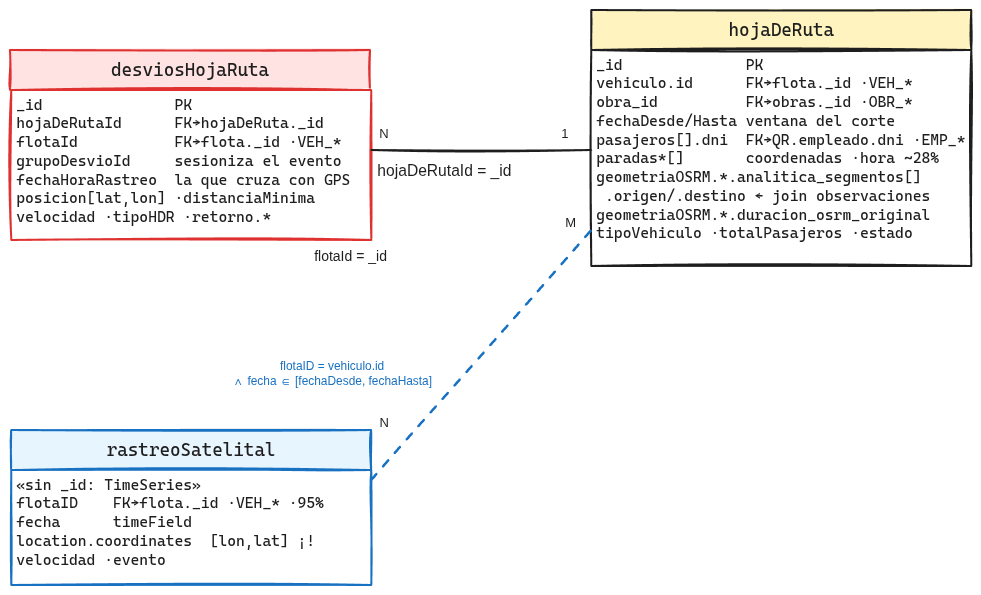
\includegraphics[width=\linewidth]{img/diagrama-colecciones.png}
  \fuente{Colecciones exportadas de MongoDB y sus claves de cruce.}
\end{column}
\begin{column}{0.36\textwidth}
  {\small
  \renewcommand{\arraystretch}{1.3}
  \begin{tabularx}{\linewidth}{@{}Yr@{}}
    \toprule
    \textbf{Colección} & \textbf{Tamaño} \\
    \midrule
    \campo{desviosHojaRuta} & 98\,MB \\
    \campo{hojaDeRuta} & 1,5\,GB \\
    \campo{rastreoSatelital} & 284\,MB \\
    \bottomrule
  \end{tabularx}}
  \vspace{0.25cm}
  \begin{itemize}\small\setlength{\itemsep}{4pt}
    \item \textbf{Desvíos}: cada vez que un vehículo está fuera de su ruta, el detector guarda su posición y la hora.
    \item \textbf{Hojas de ruta}: el plan de cada viaje: vehículo, obra de destino, pasajeros y recorrido previsto.
    \item \textbf{Rastreo satelital}: las posiciones GPS de cada vehículo durante el día, esté o no desviado.
  \end{itemize}
\end{column}
\end{columns}
\end{frame}

% ---------------------------------------------------------------------
\begin{frame}{Problemas de calidad detectados en la exploración}
  \begingroup\small
  \renewcommand{\arraystretch}{1.35}
  \begin{tabularx}{\textwidth}{@{}L{3.6cm}YY@{}}
    \toprule
    \textbf{Problema} & \textbf{Qué pasa} & \textbf{Qué hicimos} \\
    \midrule
    Coordenadas invertidas & Una colección guarda latitud y longitud en un orden y otra al revés & Se ponen todas en el mismo orden \\
    Fechas en hora UTC & Las horas vienen 3\,h adelantadas & Se pasan a hora argentina \\
    Nombre del vehículo & Cada colección lo llama distinto & Se usa un único identificador \\
    Hojas vencidas & Cada hoja vale entre dos fechas; el 61\,\% de las lecturas de desvío ocurre fuera de ese período & Se conservan, pero se marca si la hoja estaba vigente \\
    Desvíos repetidos & El mismo desvío quedó guardado varias veces, una por cada hoja de ruta del vehículo & Se deja una sola copia, la de la hoja vigente ese día \\
    Lecturas inválidas & Posición vacía $(0,0)$ o fechas imposibles & Se descartan \\
    \bottomrule
  \end{tabularx}\endgroup
\end{frame}

% =====================================================================
\section{Construcción del corpus}
% =====================================================================
\begin{frame}{Construcción del corpus: una fila por desvío}
  \begingroup\small El \textbf{corpus} es la tabla con la que aprenden los modelos: una fila por desvío, con lo que se sabía en \T\ y cuánto duró.\par\endgroup
  \vspace{0.35cm}

  \centering
  \begin{tikzpicture}[font=\scriptsize,
      paso/.style={draw=azul,fill=celestefondo,rounded corners=3pt,text width=3.0cm,minimum height=1.6cm,align=left,inner sep=4pt},
      n/.style={circle,fill=azul,text=white,font=\scriptsize\bfseries,inner sep=0pt,minimum size=0.42cm},
      fl/.style={-{Stealth[length=4pt]},azul,line width=0.8pt}]
    \foreach \i/\t/\d/\x/\y in {
      1/Limpiar lecturas/{Se descartan las que no tienen posición o tienen fecha imposible}/0/0,
      2/Armar cada desvío/{Se juntan sus lecturas: la primera es \T\ y la duración va de la primera a la última}/3.55/0,
      3/Sumar el viaje/{Se agregan los datos de la hoja de ruta: obra, vehículo y recorrido previsto}/7.1/0,
      4/Quitar repetidos/{Si un desvío quedó guardado varias veces, se deja uno}/10.65/0,
      5/Sumar lo previo/{Qué hacía el vehículo en los 10 min antes de \T: velocidad y desplazamiento}/1.775/-2.2,
      6/Sumar fecha y hora/{Hora, día de la semana y franja del día}/5.325/-2.2,
      7/Filtrar/{Quedan los desvíos con duración medible y de menos de 4\,h}/8.875/-2.2}{%
      \node[paso,anchor=north west] (p\i) at (\x,\y) {\textbf{\t}\\[2pt]{\color{gris}\d}};
      \node[n] at (p\i.north west) {\i};}
    \draw[fl] (p1) -- (p2); \draw[fl] (p2) -- (p3); \draw[fl] (p3) -- (p4);
    \draw[fl] (p4.south) |- ++(0,-0.3) -| (p5.north);
    \draw[fl] (p5) -- (p6); \draw[fl] (p6) -- (p7);
  \end{tikzpicture}
\end{frame}

% ---------------------------------------------------------------------
\begin{frame}{De los desvíos registrados al corpus}
\begin{columns}[T,onlytextwidth]
\begin{column}{0.63\textwidth}
  \centering
  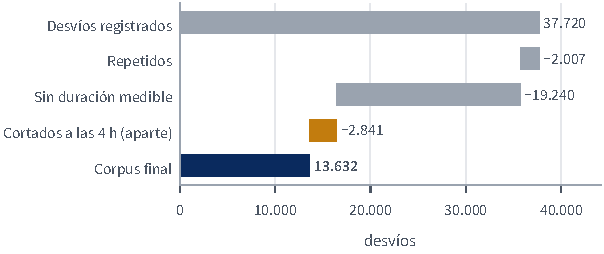
\includegraphics[width=\linewidth]{figuras/fig-embudo.pdf}
  \vspace{0.1cm}
  \begin{itemize}\footnotesize\setlength{\itemsep}{1pt}
    \item \textbf{Repetidos}: el mismo desvío guardado más de una vez.
    \item \textbf{Sin duración medible}: una sola lectura, o todas a la misma hora; no se sabe cuánto duró.
    \item \textbf{Cortados a las 4\,h}: el detector deja de medir; no se sabe cuándo terminaron. Quedan aparte.
  \end{itemize}
\end{column}
\begin{column}{0.33\textwidth}
  \vspace{0.4cm}
  \dato{13.632}{desvíos en el corpus}\par\vspace{0.4cm}
  \dato{556}{vehículos distintos}
\end{column}
\end{columns}
\end{frame}

% ---------------------------------------------------------------------
\begin{frame}{Distribución de la duración}
  \centering
  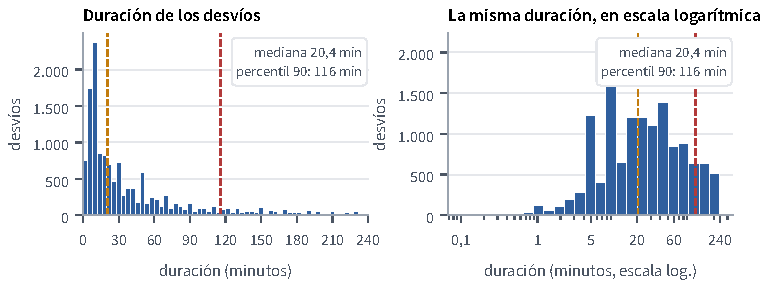
\includegraphics[width=0.9\linewidth]{figuras/fig-duracion.pdf}
  \vspace{0.1cm}
  \begin{itemize}\small\setlength{\itemsep}{1pt}
    \item La mayoría de los desvíos dura poco: la mitad dura menos de \textbf{20\,min}, pero 1 de cada 5 supera la hora.
    \item Los desvíos largos son los más difíciles de predecir. Por eso los modelos trabajan con el logaritmo de la duración (gráfico derecho), que achica la distancia entre cortos y largos.
  \end{itemize}
\end{frame}

% ---------------------------------------------------------------------
\begin{frame}{Atributos disponibles en \T}
  \begingroup\footnotesize
  \renewcommand{\arraystretch}{1.25}
  \begin{tabularx}{\textwidth}{@{}YYY@{}}
    \toprule
    \textbf{Primer ping} & \textbf{Hoja de ruta} & \textbf{Rastreo previo} \\
    {\color{gris}dónde y cómo está el vehículo} & {\color{gris}qué viaje estaba haciendo} & {\color{gris}qué venía haciendo antes} \\
    \midrule
    Distancia a la ruta & Tipo de hoja & Cantidad de lecturas GPS \\
    Velocidad & Tipo de vehículo & Velocidad media \\
    Ruta más cercana & Obra de destino & Última velocidad \\
    Latitud y longitud & Largo y duración prevista del recorrido & Minutos desde el último GPS \\
    Hora y día de la semana & Plazas y pasajeros & Distancia recorrida \\
    Franja del día & Si la hoja estaba vigente & Dirección de avance \\
    \bottomrule
  \end{tabularx}\endgroup
  \vspace{0.3cm}

  {\small 23 atributos en tres grupos, según de dónde salen. Todos se conocen en el momento de la alerta.}
\end{frame}

% ---------------------------------------------------------------------
\begin{frame}{Exploración: tipo de hoja y hora del día}
\begin{columns}[T,onlytextwidth]
\begin{column}{0.49\textwidth}
  \centering
  {\small\bfseries Duración según el tipo de hoja}\par\vspace{2pt}
  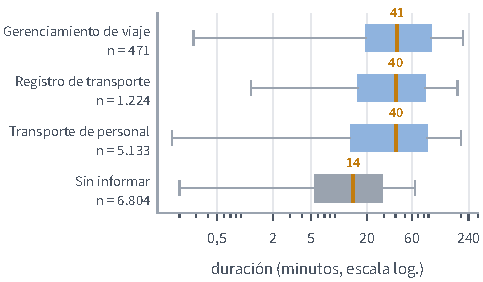
\includegraphics[width=\linewidth]{figuras/fig-tipohdr.pdf}
\end{column}
\begin{column}{0.49\textwidth}
  \centering
  {\small\bfseries Desvíos y duración según la hora}\par\vspace{2pt}
  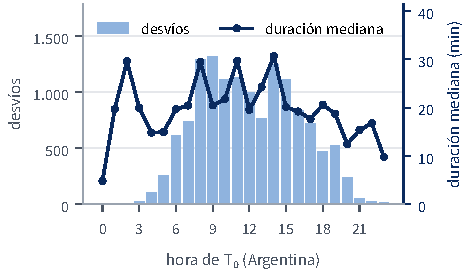
\includegraphics[width=\linewidth]{figuras/fig-hora.pdf}
\end{column}
\end{columns}
\vspace{0.15cm}
\begin{itemize}\small\setlength{\itemsep}{2pt}
  \item Cuando la hoja no dice de qué tipo es, el desvío suele ser corto: la mitad dura menos de 14\,min. Con tipo, la mitad supera los 40\,min.
  \item 9 de cada 10 desvíos ocurren entre las 6 y las 19\,h.
\end{itemize}
\fuente{Cada caja abarca la mitad central de los desvíos; la raya ámbar es la mediana, en minutos.}
\end{frame}

% =====================================================================
\section{Metodología}
% =====================================================================
\begin{frame}{Modelos comparados}
  \begingroup\small
  \renewcommand{\arraystretch}{1.35}
  \begin{tabularx}{\textwidth}{@{}L{2.9cm}YL{4.6cm}@{}}
    \toprule
    \textbf{Modelo} & \textbf{Idea} & \textbf{Configuración} \\
    \midrule
    Mediana (referencia) & Predice siempre la mediana de la duración del entrenamiento & --- \\
    Árbol de decisión & Preguntas sucesivas sobre los atributos; cada hoja predice el promedio de sus eventos & \campo{max_depth=8}, \campo{min_samples_leaf=30} \\
    Random Forest & Promedio de árboles, cada uno entrenado con una muestra al azar (con reposición) de los eventos & 200 árboles, \campo{min_samples_leaf=10} \\
    XGBoost & \emph{Boosting}: árboles chicos en secuencia, cada uno corrige el error de los anteriores & 300 árboles, \campo{learning_rate=0.05}, \campo{max_depth=4} \\
    \bottomrule
  \end{tabularx}\endgroup
  \vspace{0.3cm}
  \begin{itemize}\small\setlength{\itemsep}{2pt}
    \item Todos aprenden $z=\log(1+y)$ y se evalúan sobre $\hat{y}=e^{\hat{z}}-1$, en minutos.
    \item Parámetros elegidos a priori, sin búsqueda de hiperparámetros.
  \end{itemize}
\end{frame}

% ---------------------------------------------------------------------
\begin{frame}{Protocolo de evaluación}
\begin{columns}[T,onlytextwidth]
\begin{column}{0.5\textwidth}
  \textbf{Validación cruzada por vehículo}\par\vspace{3pt}
  {\small Se prueba siempre con vehículos que el modelo \textbf{no vio} al entrenar, como pasaría con uno nuevo. Se repite 5 veces, rotando el grupo de prueba.}\par
  \vspace{0.3cm}
  \centering
  \begin{tikzpicture}[x=0.5cm,y=0.42cm,font=\scriptsize]
    \foreach \f in {1,...,5}{%
      \node[anchor=east,gris] at (-0.2,-\f) {Partición \f};
      \foreach \v in {1,...,10}{%
        \pgfmathtruncatemacro{\g}{int((\v-1)/2)+1}
        \ifnum\g=\f \def\col{azul}\else\def\col{celeste!45}\fi
        \fill[\col] (\v-1+0.06,-\f-0.36) rectangle (\v-0.06,-\f+0.36);}}
    \node[gris,anchor=south] at (5,-0.4) {vehículos (556, en 5 grupos)};
    \fill[azul] (0,-6.4) rectangle (0.5,-6.0); \node[anchor=west] at (0.6,-6.2) {prueba};
    \fill[celeste!45] (3.6,-6.4) rectangle (4.1,-6.0); \node[anchor=west] at (4.2,-6.2) {entrenamiento};
  \end{tikzpicture}
\end{column}
\begin{column}{0.46\textwidth}
  \textbf{Métricas} {\small(en minutos)}\par\vspace{6pt}
  \begingroup\small
  \renewcommand{\arraystretch}{1.5}
  \begin{tabularx}{\linewidth}{@{}L{2.2cm}Y@{}}
    \toprule
    \textbf{MAE} & Cuántos minutos se equivoca, en promedio. \\
    \textbf{RMSE} & Igual, pero los errores grandes pesan mucho más: uno de 60\,min pesa más que seis de 10\,min. \\
    \textbf{Error mediano} & El error del caso típico: la mitad de las predicciones se equivoca menos que esto. \\
    \bottomrule
  \end{tabularx}\endgroup
  \fuente{$\text{MAE}=\frac{1}{n}\sum|y-\hat{y}|$ \quad $\text{RMSE}=\sqrt{\frac{1}{n}\sum(y-\hat{y})^2}$}
\end{column}
\end{columns}
\end{frame}

% =====================================================================
\section{Resultados}
% =====================================================================
\begin{frame}{Comparación de modelos}
\begin{columns}[c,onlytextwidth]
\begin{column}{0.57\textwidth}
  \centering
  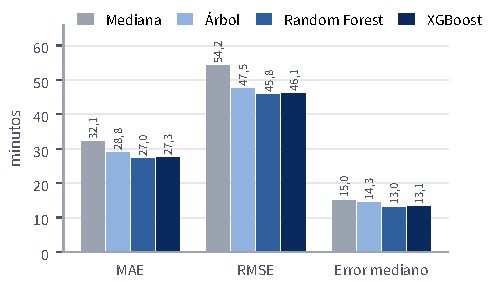
\includegraphics[width=\linewidth]{figuras/fig-metricas.pdf}
\end{column}
\begin{column}{0.41\textwidth}
  {\footnotesize
  \begin{tabular}{@{}lrrr@{}}
    \toprule
    \textbf{Modelo} & \textbf{MAE} & \textbf{RMSE} & \textbf{Mejora} \\
    \midrule
    Mediana & 32,1 & 54,2 & --- \\
    Árbol & 28,8 & 47,5 & 10\,\% \\
    Random Forest & \textbf{27,0} & \textbf{45,8} & \textbf{16\,\%} \\
    XGBoost & 27,3 & 46,1 & 15\,\% \\
    \bottomrule
  \end{tabular}}
  \fuente{Minutos. Mejora: reducción del MAE respecto de la mediana. Validación cruzada por vehículo, 13.632 eventos.}
  \vspace{0.3cm}
  {\small Los tres modelos superan a la referencia en las tres métricas. Random Forest y XGBoost quedan prácticamente empatados (0,3\,min de MAE).}
\end{column}
\end{columns}
\end{frame}

% ---------------------------------------------------------------------
\begin{frame}{Variación entre particiones}
\begin{columns}[c,onlytextwidth]
\begin{column}{0.52\textwidth}
  \centering
  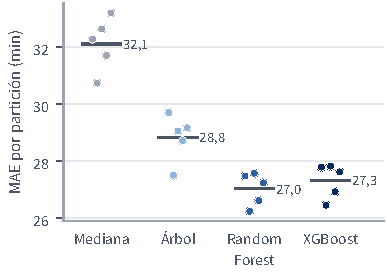
\includegraphics[width=\linewidth]{figuras/fig-particiones.pdf}
\end{column}
\begin{column}{0.44\textwidth}
  \begin{itemize}\small\setlength{\itemsep}{5pt}
    \item Cada punto es el MAE de una partición (vehículos no vistos); la línea, el promedio.
    \item Entre particiones, el MAE de Random Forest y de XGBoost varía unos 1,3\,min; entre ellos difieren 0,3\,min.
    \item Random Forest queda apenas por debajo en las cinco particiones, pero con parámetros sin ajustar la diferencia no alcanza para preferir uno.
  \end{itemize}
\end{column}
\end{columns}
\end{frame}

% ---------------------------------------------------------------------
\begin{frame}{¿Dónde se equivocan los modelos?}
\begin{columns}[c,onlytextwidth]
\begin{column}{0.57\textwidth}
  \centering
  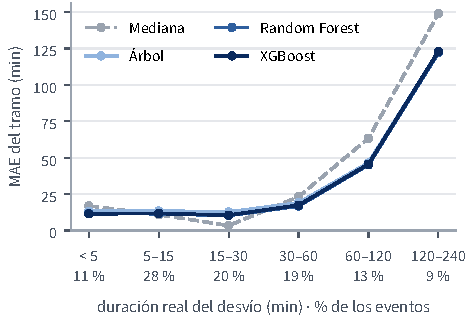
\includegraphics[width=\linewidth]{figuras/fig-error-por-duracion.pdf}
\end{column}
\begin{column}{0.41\textwidth}
  \begin{itemize}\small\setlength{\itemsep}{5pt}
    \item El error crece con la duración: los desvíos de más de 1\,h son el 22\,\% de los eventos y concentran el 64\,\% del error absoluto (Random Forest).
    \item Los modelos ganan donde la mediana falla: los muy cortos y los largos. Entre 5 y 30\,min la mediana (20\,min) ya está cerca.
    \item Por eso el RMSE es cerca de 1,7 veces el MAE.
  \end{itemize}
\end{column}
\end{columns}
\end{frame}

% ---------------------------------------------------------------------
\begin{frame}{Predicción frente a duración real}
\begin{columns}[c,onlytextwidth]
\begin{column}{0.48\textwidth}
  \centering
  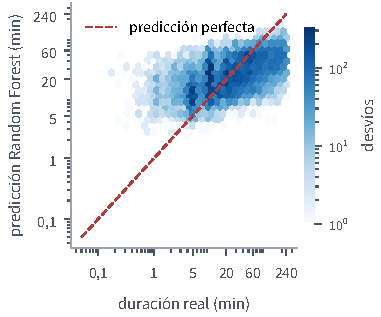
\includegraphics[width=\linewidth]{figuras/fig-real-vs-pred.pdf}
\end{column}
\begin{column}{0.48\textwidth}
  \begin{itemize}\small\setlength{\itemsep}{5pt}
    \item Random Forest, predicciones fuera de muestra; ambos ejes en escala logarítmica.
    \item El 90\,\% de las predicciones cae entre 8 y 63\,min: el modelo \textbf{acerca los extremos al centro}.
    \item Sobreestima el 99\,\% de los desvíos de menos de 5\,min y subestima el 97\,\% de los de más de 1\,h.
  \end{itemize}
\end{column}
\end{columns}
\end{frame}

% ---------------------------------------------------------------------
\begin{frame}{Importancia de las variables}
\begin{columns}[T,onlytextwidth]
\begin{column}{0.6\textwidth}
  \centering
  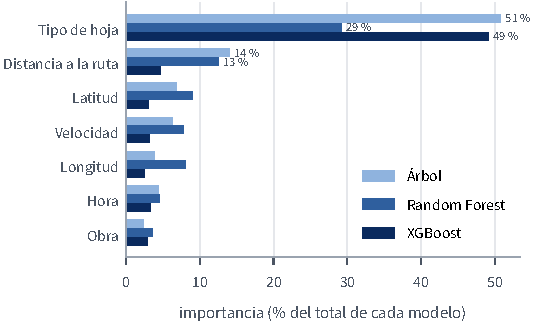
\includegraphics[width=\linewidth]{figuras/fig-importancia.pdf}
\end{column}
\begin{column}{0.38\textwidth}
  \centering
  {\small\bfseries Por grupo de atributos}\par\vspace{2pt}
  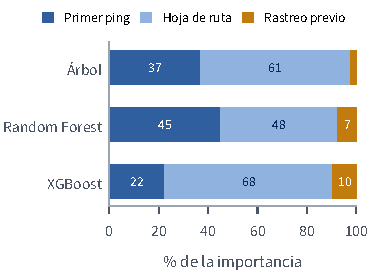
\includegraphics[width=\linewidth]{figuras/fig-importancia-grupos.pdf}\par
  \vspace{0.1cm}
  \raggedright
  \begin{itemize}\small\setlength{\itemsep}{1pt}
    \item El \textbf{tipo de hoja} es la variable más importante en los tres modelos (29 a 51\,\%).
    \item El rastreo previo pesa entre 3 y 10\,\%.
  \end{itemize}
\end{column}
\end{columns}
\fuente{Importancia por reducción del error en las divisiones (en XGBoost, ganancia), con cada modelo entrenado sobre todo el corpus. Indica qué usa el modelo, no qué causa la duración.}
\end{frame}

% ---------------------------------------------------------------------
\begin{frame}{Árbol de decisión: primeras divisiones}
\begin{columns}[c,onlytextwidth]
\begin{column}{0.68\textwidth}
  \centering
  \begin{tikzpicture}[font=\scriptsize,
      nodo/.style={draw=azul,fill=celestefondo,rounded corners=3pt,align=center,inner sep=3pt},
      raiz/.style={nodo,fill=azul,text=white},
      rama/.style={azul,line width=0.7pt}]
    \node[raiz,text width=3.6cm] (r) at (0,0) {\textbf{¿\campo{tipoHDR} informado?}\\13.632 eventos · mediana 20 min};
    \node[nodo,text width=3.1cm] (a) at (-2.55,-1.65) {\textbf{Con tipo}: 6.828 eventos\\mediana \textbf{40 min}\\¿distancia $\le$ 2.938\,m?};
    \node[nodo,text width=3.1cm] (b) at (2.55,-1.65) {\textbf{Sin tipo}: 6.804 eventos\\mediana \textbf{14 min}\\¿distancia $\le$ 1.888\,m?};
    \node[nodo,text width=1.75cm] (a1) at (-3.75,-3.35) {¿velocidad\\$\le$ 33,5?\\med. 33 min};
    \node[nodo,text width=1.75cm] (a2) at (-1.35,-3.35) {¿latitud\\$\le -38{,}75$?\\med. 50 min};
    \node[nodo,text width=1.75cm] (b1) at (1.35,-3.35) {¿latitud\\$\le -39{,}16$?\\med. 10 min};
    \node[nodo,text width=1.75cm] (b2) at (3.75,-3.35) {¿distancia\\$\le$ 13.958\,m?\\med. 16 min};
    \draw[rama] (r) -- node[left,gris,pos=0.4] {sí} (a);
    \draw[rama] (r) -- node[right,gris,pos=0.4] {no} (b);
    \draw[rama] (a) -- node[left,gris,pos=0.45] {sí} (a1); \draw[rama] (a) -- node[right,gris,pos=0.45] {no} (a2);
    \draw[rama] (b) -- node[left,gris,pos=0.45] {sí} (b1); \draw[rama] (b) -- node[right,gris,pos=0.45] {no} (b2);
    \foreach \n in {a1,a2,b1,b2}{\draw[gris,dashed] (\n.south) -- ++(0,-0.35) node[below,inner sep=1pt] {$\vdots$};}
  \end{tikzpicture}
\end{column}
\begin{column}{0.3\textwidth}
  \begin{itemize}\small\setlength{\itemsep}{5pt}
    \item La raíz separa el corpus en dos mitades con medianas muy distintas: 40 frente a 14 min.
    \item El segundo nivel usa la distancia a la ruta en ambas ramas.
    \item El árbol completo llega a 8 niveles.
  \end{itemize}
\end{column}
\end{columns}
\end{frame}

% ---------------------------------------------------------------------
\begin{frame}{Aporte de cada grupo de atributos}
\begin{columns}[c,onlytextwidth]
\begin{column}{0.5\textwidth}
  \centering
  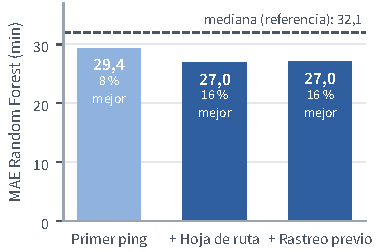
\includegraphics[width=\linewidth]{figuras/fig-ablacion.pdf}
\end{column}
\begin{column}{0.46\textwidth}
  {\small Random Forest entrenado sumando los grupos de atributos de a uno:}
  \begin{itemize}\small\setlength{\itemsep}{4pt}
    \item Solo con el \textbf{primer ping} ya mejora a la mediana.
    \item La \textbf{hoja de ruta} baja el MAE de 29,4 a 27,0 minutos.
    \item El \textbf{rastreo previo} no cambia el resultado (27,0): el 42\,\% de los eventos no tiene GPS previo y, cuando lo hay, son una o dos lecturas.
  \end{itemize}
\end{column}
\end{columns}
\end{frame}

% =====================================================================
\section{Conclusiones}
% =====================================================================
\begin{frame}{Conclusiones}
  \begin{columns}[T,onlytextwidth]
  \begin{column}{0.485\textwidth}
    \begin{exampleblock}{Hay señal}
      \small Con la información de \T\ los tres modelos superan a la mediana en vehículos no vistos. El mejor reduce el MAE de 32,1 a 27,0 minutos y el RMSE de 54,2 a 45,8 (cerca de 16\,\%).
    \end{exampleblock}
    \vspace{0.2cm}
    \begin{block}{Dónde está la señal}
      \small En el tipo de hoja y en el primer ping (distancia a la ruta, posición, velocidad). El rastreo previo casi no aporta.
    \end{block}
  \end{column}
  \begin{column}{0.485\textwidth}
    \begin{alertblock}{Pero la mejora es modesta}
      \small El mejor modelo se equivoca 27 minutos en promedio, cuando la duración mediana de un desvío es de 20 minutos. El error se concentra en los desvíos largos.
    \end{alertblock}
    \vspace{0.2cm}
    \begin{block}{Random Forest y XGBoost}
      \small Quedan empatados dentro de la variación entre particiones, ambos sin ajuste de parámetros.
    \end{block}
  \end{column}
  \end{columns}
\end{frame}

% ---------------------------------------------------------------------
\begin{frame}{Limitaciones y trabajo futuro}
\begin{columns}[T,onlytextwidth]
\begin{column}{0.485\textwidth}
  \textbf{\color{rojo}Limitaciones}
  \begin{itemize}\small\setlength{\itemsep}{3pt}
    \item Los 2.841 desvíos que llegan al tope de 4\,h quedan fuera: el error medido es optimista.
    \item Parámetros sin ajustar en todos los modelos.
    \item Categorías codificadas como enteros, con un orden que no tienen.
    \item El 61\,\% de los desvíos cae fuera de la vigencia de su hoja.
    \item El rastreo empieza un mes después que los desvíos.
  \end{itemize}
\end{column}
\begin{column}{0.485\textwidth}
  \textbf{\color{verde}Trabajo futuro}
  \begin{itemize}\small\setlength{\itemsep}{3pt}
    \item Tratar los eventos del tope como datos censurados (modelos de supervivencia).
    \item Una etapa previa que clasifique desvíos cortos y largos.
    \item Búsqueda de hiperparámetros con validación anidada.
    \item Reportar el error por segmento operativo: tipo de vehículo, franja horaria, obra.
  \end{itemize}
\end{column}
\end{columns}
\end{frame}

% ---------------------------------------------------------------------
{\setbeamertemplate{footline}{}
\begin{frame}[noframenumbering]
  \begin{tikzpicture}[remember picture,overlay]
    \fill[azul] (current page.south west) rectangle (current page.north east);
    \node[text=white,font=\Huge\bfseries] at ([yshift=0.9cm]current page.center) {Muchas gracias};
    \node[text=celeste,font=\large] at ([yshift=-0.05cm]current page.center) {¿Preguntas?};
    \node[text=white!80!azul,font=\small,align=center] at ([yshift=-1.4cm]current page.center)
      {Código, notebook e informes:\\[2pt]{\ttfamily github.com/sebareibold/prediccion-duracion-desvios}};
    \node[text=white!65!azul,font=\scriptsize] at ([yshift=0.6cm]current page.south) {Grupo 5 · Laboratorio de Inteligencia Artificial · FAI · UNComa};
  \end{tikzpicture}
\end{frame}}

\end{document}
